\documentclass[xcolor={dvipsnames}]{beamer}
\usepackage{pgfplots}
\pgfplotsset{compat=1.11}
\usepgfplotslibrary{fillbetween}

\begin{document}
\begin{frame}
\centering
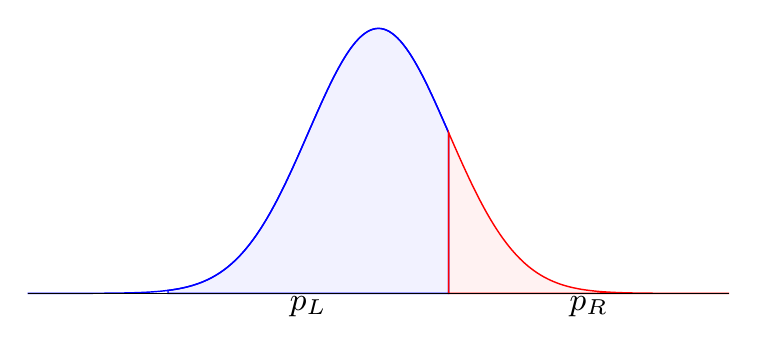
\begin{tikzpicture}[scale=1.3]
\begin{axis}[axis lines=none, xtick=\empty, ytick=\empty,xmin=0,xmax=10,ymax=1,domain=0:10,
          restrict y to domain=0:1]
\addplot[blue,samples=100,domain=0:6]  {1/2*exp((-(x-5)^2)/2)} ;
\addplot[blue,fill=blue,fill opacity=0.05,samples=100,domain=2:6]  {1/2*exp((-(x-5)^2)/2)} \closedcycle;
\addplot[red,fill=red,fill opacity=0.05,samples=100,domain=6:10]  {1/2*exp((-(x-5)^2)/2)} \closedcycle;;
\addplot[black,samples=100,domain=0:10]  {0} node[above]{};
\node  at (axis cs: 4, -0.025) {\small{$p_L$}};
\node  at (axis cs: 8, -0.025) {\small{$p_R$}};
%\addplot[blue,domain=1/2^6:10,samples=100]  {log2(x)} node[above left] {$y=\log_2(x)$};
\end{axis}
\end{tikzpicture}
\end{frame}
\end{document}